\chapter{Normalisation fit}
\label{sec:Normalisationfit}

This chapter describes the analysis of the normalisation channel \LbToLcmunu (\LcTopKpi) resulting in the signal yield \NLc for the calculation of \R. The method is different to the one in the signal channel \LbToDpmunuX due to several reasons:
The final state particles of the subdecay \LcTopKpi are all reconstructed. 
It is thus possible to see a clear \Lc mass peak as shown in figure \ref{fig:plot_Lc_M}.
The small sidebands indicate a small combinatorial background concerning the subdecay \LcTopKpi.
Background coming from a random combination of a \Lc with a muon can be estimated by a look at the WS final states combinations \Lc\mup.
Since a \Lb can't decay into a \Lc\mup due to charge conservation, this unphysical combination gives a good hint for randomly combined \Lc\mun.
The second reason why a different method is chosen compared to the \LbToDpmunuX channel is the fact that the \Lb can decay in several excited \Lc states (in the following denoted as \Lcstar for any excited \Lc state).
It has been shown in \ref{SL_Vub} that the \LbToLcmunu data is saturated by the decays \decay{\Lb}{\LcstarRes{(2595)}\mun\neumb} and \decay{\Lb}{\LcstarRes{(2625)}\mun\neumb}.
These excited \Lcstar instantly decay for instance in \Lc\pip\pim. 
If these two pions aren't reconstructed, this decay can't be distinguished by its topology.
That's why a different approach for the determination of \NLc has to be chosen.
The solution of the latter problem is to fit the corrected \pKpi\mun, i.e the visible \Lb mass.
An explanation for this choice and the description of the fit is given in section \ref{sec:Normalisationfit}.
\begin{figure}[hptb]
    \centering
	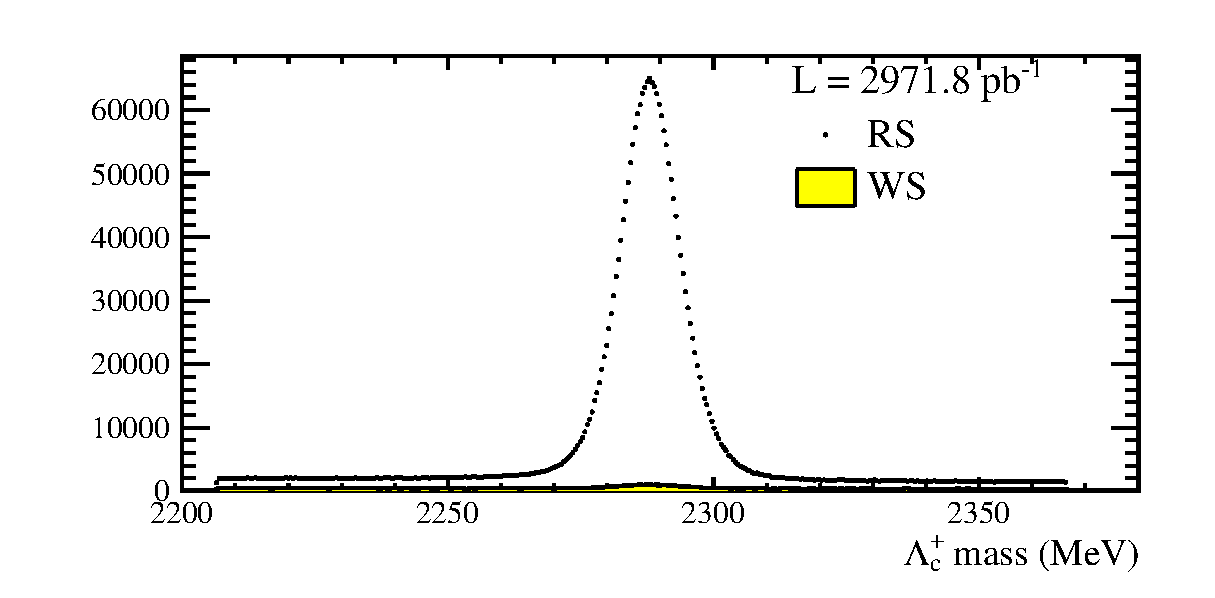
\includegraphics[width=\textwidth]{LbToLc/plots/data/Lc_M}	
	\caption{Plot of the invariant \pKpi mass. A clear mass peak identified as the \Lc can be seen. The yellow shaded area shows events with the WS combination \Lc\mup.}
	\label{fig:plot_Lc_M}
\end{figure}

\section{Reduction of non \Lc background}
As already mentioned the reconstructed \pKpi mass delivers a nice peak forming the hadronically decaying \Lc nicely seen in figure \ref{fig:plot_Lc_M}. 
Events being outside of this peak can be explained by a random combination of proton, kaon and pion and thus not being decay remnants of the \Lc.
Nonetheless there is also a certain amount of this ``combinatoric" background in the peak region.
It is statistically eliminated by a sideband subtraction (see section \ref{sec:Sidebandsubtraction}.
As signal band

\section{Fit of the \pKpi\mun corrected mass}
\label{sec:FitCorrectedMass}
